\documentclass[a4paper]{article}
\usepackage[warn]{mathtext}
\usepackage{graphicx}
\usepackage{wrapfig}
\usepackage{enumitem}
\usepackage[center]{caption}
\usepackage[english, russian]{babel}
\usepackage{amsmath}
\usepackage{amssymb}
\usepackage{geometry}
\usepackage{longtable}
\usepackage{booktabs}
\setcounter{totalnumber}{5}

\geometry{verbose, a4paper, tmargin=2cm, bmargin=2cm, lmargin=2.0cm, rmargin=2.0cm}

\begin{document}
	
	\begin{titlepage}
		\centering
		{\scshape\Large МОСКОВСКИЙ ФИЗИКО-ТЕХНИЧЕСКИЙ ИНСТИТУТ \\
			(НАЦИОНАЛЬНЫЙ ИССЛЕДОВАТЕЛЬСКИЙ УНИВЕРСИТЕТ)\\
			Физтех-школа аэрокосмических технологий}
		
		\vspace{4cm}
		{\LARGE Отчет о выполнении лабораторной работы 3.4.4}
		\vspace{1cm}
		
		{\huge\bf Петля гистерезиса (статический метод)}
		
		\vspace{1cm}
		\vfill
		
		\begin{flushright}
			{\LARGE Губарев Никита, Б03-502}
		\end{flushright}
		\vfill 
		\today
	\end{titlepage}
	
	\tableofcontents
	
	\section{Аннотация}
	
	\textbf{Цель работы:} наблюдение начальной кривой намагничивания ферромагнетика и предельной петли гистерезиса; определение основных магнитных характеристик материала: коэрцитивной силы $H_c$, остаточной индукции $B_r$, индукции насыщения $B_s$ и максимальной дифференциальной магнитной проницаемости $\mu_{\text{диф}}$.
	
	\textbf{В работе используются:} генератор токов намагничивания (ГТН), тороид, калибровочный соленоид, баллистический гальванометр с осветителем и шкалой, амперметр, магазин сопротивлений $R_M$, ЛАТР, разделительный трансформатор, ключи и переключатели $\Pi_1$, $\Pi_2$, $K_0$, $K_1$.
	
	\section{Описание работы}
	
	\subsection{Теоретические сведения}
	
	\subsubsection{Ферромагнетизм и доменная структура}
	
	Ферромагнетиками называют вещества, способные обладать спонтанной намагниченностью в отсутствие внешнего магнитного поля. К ним относятся железо, никель, кобальт, гадолиний и их многочисленные сплавы. Микроскопической причиной ферромагнетизма является обменное взаимодействие электронов соседних атомов, имеющее электростатическую природу и энергетически выгодное при параллельной ориентации спинов.
	
	Даже в отсутствие внешнего поля ферромагнетик может быть в целом не намагничен из-за разбиения на области самопроизвольной намагниченности — \textbf{домены}. В каждом домене магнитные моменты атомов ориентированы одинаково, но направления намагниченности разных доменов различны, что минимизирует полную энергию системы.
	
	\subsubsection{Кривая намагничивания и гистерезис}
	
	Связь между магнитной индукцией $B$ и напряжённостью магнитного поля $H$ в ферромагнетике неоднозначна: индукция зависит не только от текущего значения напряжённости, но и от предыстории образца. Это явление называется \textbf{гистерезисом}.
	
	При монотонном увеличении $H$ от нуля (для размагниченного образца) зависимость $B(H)$ описывается \textbf{начальной кривой намагничивания}. На ней выделяют несколько характерных участков:
	
	\begin{enumerate}
		\item \textbf{Область обратимого намагничивания} (малые $H$): $B = \mu_{\text{нач}} \mu_0 H$.
		\item \textbf{Область нелинейного роста}: наклон кривой увеличивается.
		\item \textbf{Область максимальной крутизны}: необратимые смещения доменных стенок, преодолевающих препятствия; скачки Баркгаузена.
		\item \textbf{Область насыщения}: все домены ориентированы по полю. Дальнейший рост $B$ происходит только за счёт $H$: $B = \mu_0 H + \mu_0 M_s$. Это значение называют \textbf{индукцией насыщения} $B_s$.
	\end{enumerate}
	
	При уменьшении $H$ после достижения насыщения индукция убывает не по начальной кривой, а по кривой, лежащей выше. При $H = 0$ в образце сохраняется \textbf{остаточная индукция} $B_r$. Для полного размагничивания необходимо приложить обратное поле $-H_c$; величину $H_c$ называют \textbf{коэрцитивной силой}. Замкнутая кривая при циклическом перемагничивании до насыщения в обе стороны называется \textbf{предельной петлёй гистерезиса}.
	
	\subsubsection{Дифференциальная магнитная проницаемость}
	
	Наклон кривой намагничивания характеризуется \textbf{дифференциальной магнитной проницаемостью}:
	\begin{equation}
		\mu_{\text{диф}} = \frac{1}{\mu_0} \frac{dB}{dH}.
		\label{eq:mu_diff}
	\end{equation}
	
	\subsection{Метод измерения}
	
	\subsubsection{Схема измерений}
	
	Для измерения зависимости $B(H)$ используется тороидальный образец с двумя обмотками: намагничивающей ($N_{t0}$ витков) и измерительной ($N_{t1}$ витков). Напряжённость магнитного поля в тороиде:
	\begin{equation}
		H \approx \frac{N_{t0}}{\pi D} I,
		\label{eq:H}
	\end{equation}
	где $D$ — средний диаметр тора.
	
	При скачкообразном изменении тока $\Delta I$ в измерительной обмотке возникает ЭДС индукции, и баллистический гальванометр регистрирует отклонение $\Delta x \propto \Delta B$.
	
	\subsubsection{Калибровка гальванометра}
	
	Исключая баллистическую постоянную $b$ из уравнений для тороида и соленоида, получаем:
	\begin{equation}
		\Delta B = \mu_0 \left(\frac{d_c}{d_t}\right)^2 \frac{N_{c1} N_{c0}}{N_{t1}} \frac{R}{R_c} \frac{1}{l_c} \frac{\Delta I_c}{\Delta x_c} \Delta x.
		\label{eq:dB}
	\end{equation}
	
	\textbf{Замечание о сопротивлениях.} При $R_M = 60$ Ом и $R_C = 60$ Ом уменьшение $R_M$ на $R_C$ привело бы к полному выводу магазина из цепи. Поэтому \textbf{мы уменьшили сопротивление не на 60 Ом, а на 50 Ом}, установив $R'_M = 10$ Ом. Сопротивлениями $R_T$ и $R_0$ пренебрегаем.
	
	\section{Методика измерений}
	
	\subsection{О порядке переключения $\Pi_1$ и $\Pi_2$}
	
	Переключатель $\Pi_1$ меняет направление тока в \emph{намагничивающей} обмотке (знак $H$), а $\Pi_2$ — направление тока в \emph{измерительной} цепи (знак регистрируемого отклонения). Переключатель $\Pi_2$ \textbf{не влияет} на состояние образца.
	
	\textbf{Правильная процедура обхода}:
	\begin{enumerate}
		\item Сегмент 1 (11\,$\to$\,0): $\Pi_1$, $\Pi_2$ в исходном положении; $H > 0$, $B$ убывает от $+B_s$ к $+B_r$.
		\item Переключаем \textbf{только} $\Pi_1$. Сегмент 2 (0\,$\to$\,11): $H < 0$, $B$ продолжает убывать.
		\item Переключаем \textbf{только} $\Pi_2$. Сегмент 3 (11\,$\to$\,0): $H$ отрицательно, но $B$ теперь \emph{растёт} — идём по восходящей ветви.
		\item Переключаем \textbf{только} $\Pi_1$. Сегмент 4 (0\,$\to$\,11): $H > 0$, $B$ растёт до $+B_s$.
	\end{enumerate}
	
	\textbf{Почему нельзя переключать оба одновременно.} Если в точке $C'$ переключить $\Pi_1$ и $\Pi_2$ одновременно, то $\Pi_1$ мгновенно меняет знак $H$ ($-H_{\max} \to +H_{\max}$), и образец «соскакивает» с состояния $-B_s$ снова на нисходящую ветвь. Сегменты 3 и 4 оказываются зеркальными копиями сегментов 1 и 2 — образец дважды проходит одну и ту же половину петли.
	
	\section{Результаты измерений}
	
	\subsection{Токи на ступенях ГТН}
	
	\begin{table}[h]
		\centering
		\caption{Значения тока на ступенях ГТН}
		\label{tab:currents}
		\begin{tabular}{|c|c|c|c|c|c|c|c|c|c|c|c|c|}
			\hline
			Ступень & 0 & 1 & 2 & 3 & 4 & 5 & 6 & 7 & 8 & 9 & 10 & 11 \\
			\hline
			$I$, А & 0 & 0.0152 & 0.0279 & 0.0389 & 0.0442 & 0.0556 & 0.0663 & 0.0945 & 0.1567 & 0.2498 & 0.5128 & 1.4560 \\
			\hline
			$\delta I$, А & \multicolumn{12}{c|}{$0.001$ для всех ступеней} \\
			\hline
		\end{tabular}
	\end{table}
	
	\subsection{Первый проход (правильный, $R_M = 50$ Ом)}
	
	\begin{longtable}{|c|c|c|}
		\hline
		Откуда & Куда & Отклонение, см ($\pm 0.2$ см) \\
		\hline
		11 & 10 & 20.6 \\ \hline
		10 & 9 & 19.4 \\ \hline
		9 & 8 & 11.7 \\ \hline
		8 & 7 & 8.1 \\ \hline
		7 & 6 & 4.1 \\ \hline
		6 & 5 & 2.5 \\ \hline
		5 & 4 & 2.3 \\ \hline
		4 & 3 & 1.3 \\ \hline
		3 & 2 & 1.6 \\ \hline
		2 & 1 & 1.8 \\ \hline
		1 & 0 & 4.5 \\ \hline
		0 & 1 & 8.1 \\ \hline
		1 & 2 & 11.1 \\ \hline
		2 & 3 & 24.6 \\ \hline
		3 & 4 & 17.5 \\ \hline
		4 & 5 & 29.2 \\ \hline
		5 & 6 & 16.0 \\ \hline
		6 & 7 & 25.6 \\ \hline
		7 & 8 & 26.2 \\ \hline
		8 & 9 & 18.2 \\ \hline
		9 & 10 & 23.0 \\ \hline
		10 & 11 & 20.9 \\ \hline
		11 & 10 & 20.1 \\ \hline
		10 & 9 & 19.2 \\ \hline
		9 & 8 & 11.6 \\ \hline
		8 & 7 & 11.2 \\ \hline
		7 & 6 & 3.9 \\ \hline
		6 & 5 & 2.9 \\ \hline
		5 & 4 & 1.9 \\ \hline
		4 & 3 & 0.7 \\ \hline
		3 & 2 & 1.0 \\ \hline
		2 & 1 & 1.3 \\ \hline
		1 & 0 & 3.8 \\ \hline
		0 & 1 & 8.3 \\ \hline
		1 & 2 & 11.2 \\ \hline
		2 & 3 & 24.4 \\ \hline
		3 & 4 & 17.9 \\ \hline
		4 & 5 & 28.9 \\ \hline
		5 & 6 & 16.3 \\ \hline
		6 & 7 & 26.0 \\ \hline
		7 & 8 & 26.3 \\ \hline
		8 & 9 & 18.2 \\ \hline
		9 & 10 & 23.1 \\ \hline
		10 & 11 & 20.9 \\ \hline
		\caption{Первый проход (правильный): переключали только $\Pi_2$ в середине}
		\label{tab:first_attempt}
	\end{longtable}
	
	\subsection{Второй проход (ошибочный, $R_M = 60$ Ом)}
	
	\begin{longtable}{|c|c|c|}
		\hline
		Откуда & Куда & Отклонение, см ($\pm 0.2$ см) \\
		\hline
		11 & 10 & 20.3 \\ \hline
		10 & 9 & 17.9 \\ \hline
		9 & 8 & 11.6 \\ \hline
		8 & 7 & 9.2 \\ \hline
		7 & 6 & 4.3 \\ \hline
		6 & 5 & 2.5 \\ \hline
		5 & 4 & 1.4 \\ \hline
		4 & 3 & 0.9 \\ \hline
		3 & 2 & 1.1 \\ \hline
		2 & 1 & 1.4 \\ \hline
		1 & 0 & 2.6 \\ \hline
		0 & 1 & 7.7 \\ \hline
		1 & 2 & 10.4 \\ \hline
		2 & 3 & 22.8 \\ \hline
		3 & 4 & 16.2 \\ \hline
		4 & 5 & 26.2 \\ \hline
		5 & 6 & 14.8 \\ \hline
		6 & 7 & 23.5 \\ \hline
		7 & 8 & 23.9 \\ \hline
		8 & 9 & 16.9 \\ \hline
		9 & 10 & 21.0 \\ \hline
		10 & 11 & 19.0 \\ \hline
		11 & 10 & 19.1 \\ \hline
		10 & 9 & 20.4 \\ \hline
		9 & 8 & 12.1 \\ \hline
		8 & 7 & 10.0 \\ \hline
		7 & 6 & 3.7 \\ \hline
		6 & 5 & 1.5 \\ \hline
		5 & 4 & 1.3 \\ \hline
		4 & 3 & 0.8 \\ \hline
		3 & 2 & 1.2 \\ \hline
		2 & 1 & 1.0 \\ \hline
		1 & 0 & 2.4 \\ \hline
		0 & 1 & 7.8 \\ \hline
		1 & 2 & 10.7 \\ \hline
		2 & 3 & 24.3 \\ \hline
		3 & 4 & 16.6 \\ \hline
		4 & 5 & 27.8 \\ \hline
		5 & 6 & 15.1 \\ \hline
		6 & 7 & 25.0 \\ \hline
		7 & 8 & 25.2 \\ \hline
		8 & 9 & 17.1 \\ \hline
		9 & 10 & 21.9 \\ \hline
		10 & 11 & 19.8 \\ \hline
		\caption{Второй проход (ошибочный): переключали $\Pi_1$ и $\Pi_2$ одновременно}
		\label{tab:second_attempt}
	\end{longtable}
	
	\subsection{Калибровка гальванометра}
	
	\begin{table}[h]
		\centering
		\caption{Калибровка гальванометра ($R'_M = 10$ Ом)}
		\label{tab:calib}
		\begin{tabular}{|c|c|c|c|}
			\hline
			$I_{\max}$, А & $x_1$, см & $x_0$, см & $\Delta x_c$, см \\
			\hline
			$1.4566 \pm 0.001$ & $4.1 \pm 0.2$ & $-5.2 \pm 0.2$ & $9.3 \pm 0.4$ \\
			\hline
		\end{tabular}
	\end{table}
	
	\subsection{Начальная кривая намагничивания}
	
	\begin{table}[h]
		\centering
		\caption{Начальная кривая намагничивания}
		\label{tab:initial}
		\begin{tabular}{|c|c|c|}
			\hline
			Откуда & Куда & Отклонение, см ($\pm 0.2$ см) \\
			\hline
			0 & 1 & 3.4 \\ \hline
			1 & 2 & 6.6 \\ \hline
			2 & 3 & 11.5 \\ \hline
			3 & 4 & 5.9 \\ \hline
			4 & 5 & 11.3 \\ \hline
			5 & 6 & 8.6 \\ \hline
			6 & 7 & 16.8 \\ \hline
			7 & 8 & 21.0 \\ \hline
			8 & 9 & 16.1 \\ \hline
			9 & 10 & 21.0 \\ \hline
			10 & 11 & 19.4 \\ \hline
		\end{tabular}
	\end{table}
	
	\section{Обработка результатов}
	
	\subsection{Параметры установки}
	
	\begin{table}[h]
		\centering
		\caption{Параметры установки}
		\label{tab:params}
		\begin{tabular}{|l|c|c|}
			\hline
			Параметр & Обозначение & Значение \\
			\hline
			Число витков намагничивающей обмотки тороида & $N_{t0}$ & 1750 \\
			\hline
			Число витков измерительной обмотки тороида & $N_{t1}$ & 300 \\
			\hline
			Средний диаметр тора & $D$ & 10 см \\
			\hline
			Диаметр поперечного сечения тора & $d_t$ & 1 см \\
			\hline
			Число витков намагничивающей обмотки соленоида & $N_{c0}$ & 825 \\
			\hline
			Число витков измерительной обмотки соленоида & $N_{c1}$ & 435 \\
			\hline
			Длина соленоида & $l_c$ & 80 см \\
			\hline
			Диаметр соленоида & $d_c$ & 7 см \\
			\hline
			Сопротивление соленоида & $R_C$ & 60 Ом \\
			\hline
			Сопротивление магазина (первый проход) & $R_M$ & 50 Ом \\
			\hline
			Сопротивление магазина (второй проход) & $R_M$ & 60 Ом \\
			\hline
			Сопротивление магазина (калибровка) & $R'_M$ & 10 Ом \\
			\hline
			Сопротивления $R_T$, $R_0$ & & $\approx 0$ (пренебрегаем) \\
			\hline
		\end{tabular}
	\end{table}
	
	\subsection{Численные параметры расчёта}
	
	\begin{table}[h]
		\centering
		\caption{Параметры расчёта и их погрешности}
		\label{tab:numerical_params}
		\begin{tabular}{|l|c|c|c|}
			\hline
			Параметр & Обозначение & Значение & Погрешность \\
			\hline
			Сопротивление цепи (первый проход) & $R$ & 50 Ом & --- \\
			\hline
			Отношение $R/R_c$ (первый) & & 0.714 & --- \\
			\hline
			Отношение $R/R_c$ (второй) & & 0.857 & --- \\
			\hline
			Коэффициент пересчёта (первый) & $K_1$ & $10.30 \cdot 10^{-3}$ Тл/см & $0.22 \cdot 10^{-3}$ Тл/см \\
			\hline
			Коэффициент пересчёта (второй) & $K_2$ & $12.36 \cdot 10^{-3}$ Тл/см & $0.27 \cdot 10^{-3}$ Тл/см \\
			\hline
			Погрешность $\Delta B$ на шаг & $\delta(\Delta B)$ & --- & 2.06 мТл \\
			\hline
			Погрешность $H$ & $\delta H$ & --- & 5.57 А/м \\
			\hline
			Относительная погрешность $K$ & $\delta K/K$ & --- & 2.15\% \\
			\hline
		\end{tabular}
	\end{table}
	
	\subsection{Проверка правильности обхода по суммам $\Delta x$}
	
	\textbf{Первый проход} (флип только $\Pi_2$):
	\[
	\sum_1 = 77.9 \text{ см}, \quad \sum_3 = 77.6 \text{ см}, \quad
	\sum_2 = 220.4 \text{ см}, \quad \sum_4 = 221.5 \text{ см}.
	\]
	Отклонение $\sum_1$ от $\sum_3$: 0.4\,\%; $\sum_2$ от $\sum_4$: 0.5\,\%. \textbf{Петля практически замкнута — обход правильный.}
	
	\textbf{Второй проход} (флип $\Pi_1$ и $\Pi_2$ одновременно):
	\[
	\sum_1 = 73.2 \text{ см}, \quad \sum_3 = 73.5 \text{ см}, \quad
	\sum_2 = 202.4 \text{ см}, \quad \sum_4 = 211.3 \text{ см}.
	\]
	Отклонение $\sum_1$ от $\sum_3$: 0.4\,\%; но $\sum_2$ от $\sum_4$: \textbf{4.3\,\%} — заметная асимметрия, указывающая на ошибочный обход.
	
	\textbf{Физический аргумент} (главный): при двойном флипе $\Pi_1$ мгновенно перебрасывает $H$ из $-H_{\max}$ в $+H_{\max}$, образец «соскакивает» на ту же (нисходящую) ветвь петли, и сегменты 3--4 оказываются зеркальными копиями сегментов 1--2. Поэтому для определения характеристик используется \textbf{первый проход}.
	
	\subsection{Итоговые характеристики материала}
	
	\begin{table}[h]
		\centering
		\caption{Итоговые характеристики (по правильному проходу)}
		\label{tab:numerical_results}
		\begin{tabular}{|l|c|c|c|}
			\hline
			Характеристика & Обозначение & Значение & Справочно \\
			\hline
			Индукция насыщения & $B_s$ & $(1.54 \pm 0.04)$ Тл & 1.5--2.1 Тл \\
			\hline
			Остаточная индукция & $B_r$ & $(0.73 \pm 0.02)$ Тл & 0.6--1.0 Тл \\
			\hline
			Коэрцитивная сила & $|H_c|$ & $(246 \pm 10)$ А/м & 100--500 А/м \\
			\hline
			Амплитуда $B$ (ошибочный проход) & $B_{\max}^{\text{wrong}}$ & $1.76$ Тл & --- \\
			\hline
		\end{tabular}
	\end{table}
	
	Все три характеристики попадают в справочные диапазоны для мягкой стали.
	
	\subsection{Как считались погрешности}
	
	\textbf{Прямые измерения:}
	\begin{itemize}
		\item Ток: $\delta I = 0.001$ А (по паспорту амперметра);
		\item Отклонение зайчика: $\delta x = 0.2$ см = 2 мм.
	\end{itemize}
	
	\textbf{Напряжённость поля:}
	\[
	\delta H = \frac{N_{t0}}{\pi D} \delta I = \frac{1750}{\pi \cdot 0.1} \cdot 0.001 \approx 5.57 \ \text{А/м}.
	\]
	
	\textbf{Изменение индукции на один шаг:}
	\[
	\delta(\Delta B) = K_1 \cdot \delta x = 10.30 \cdot 10^{-3} \cdot 0.2 \approx 2.06 \ \text{мТл}.
	\]
	
	\textbf{Погрешность коэффициента $K$:}
	\[
	\frac{\delta K}{K} = \sqrt{\left(\frac{\delta I_c}{I_c}\right)^2 + \left(\frac{\delta x_c}{x_c}\right)^2}
	= \sqrt{\left(\frac{0.001}{1.4566}\right)^2 + \left(\frac{0.2}{9.3}\right)^2} \approx 0.0215 = 2.15\%.
	\]
	\[
	\delta K_1 \approx K_1 \cdot 0.0215 \approx 0.22 \cdot 10^{-3} \ \text{Тл/см}.
	\]
	
	\textbf{Накопленная погрешность $B$:}
	\[
	\delta B_{\text{накоп}} = \sqrt{n} \cdot \delta(\Delta B), \quad n \approx 44 \Rightarrow \delta B \approx 0.014 \ \text{Тл}.
	\]
	Плюс систематическая от неточности $K$: $(\delta K/K) \cdot B_s \approx 0.033$ Тл.
	\[
	\delta B_s = \sqrt{(0.014)^2 + (0.033)^2} \approx 0.04 \ \text{Тл}.
	\]
	
	\textbf{Погрешность $H_c$:}
	\[
	\delta H_c = \sqrt{\delta H^2 + \left(\frac{\delta B}{(\mu_0\mu_{\text{диф}})}\right)^2} \approx 10 \ \text{А/м}.
	\]
	
	\subsection{Сводная таблица погрешностей}
	
	\begin{table}[h]
		\centering
		\caption{Сводка погрешностей}
		\label{tab:errors_summary}
		\begin{tabular}{|l|c|c|}
			\hline
			Величина & Обозначение & Значение \\
			\hline
			Ток на ступени & $\delta I$ & 0.001 А \\
			\hline
			Отклонение зайчика & $\delta x$ & 0.2 см \\
			\hline
			Напряжённость поля & $\delta H$ & 5.57 А/м \\
			\hline
			Изменение индукции на шаг & $\delta(\Delta B)$ & 2.06 мТл \\
			\hline
			Коэффициент пересчёта & $\delta K_1$ & $0.22\cdot 10^{-3}$ Тл/см \\
			\hline
			Накопленная $B$ (полная петля) & $\delta B_{\text{накоп}}$ & 0.014 Тл \\
			\hline
			Индукция насыщения & $\delta B_s$ & 0.04 Тл \\
			\hline
			Остаточная индукция & $\delta B_r$ & 0.02 Тл \\
			\hline
			Коэрцитивная сила & $\delta H_c$ & 10 А/м \\
			\hline
			Тепловой дрейф (большие токи) & $\delta_{\text{терм}}$ & $\approx 3$--$5\%$ \\
			\hline
		\end{tabular}
	\end{table}
	
	\section{Обсуждение результатов}
	
	\subsection{О правильности обхода петли}
	
	Первый проход (флип только $\Pi_2$) даёт замкнутую симметричную петлю; второй (флип $\Pi_1+\Pi_2$) — асимметричную (расхождение $\sum_2$ и $\sum_4$ достигает 4.3\,\%). Поэтому для определения характеристик используется \textbf{первый проход}. Амплитуда индукции в ошибочном проходе оказалась завышенной ($\pm 1.76$ Тл) из-за большего $K_2$ (при $R_M = 60$ Ом) — но это артефакт неправильного обхода, а не свойство материала.
	
	\subsection{Влияние тепловых эффектов}
	
	При больших токах ($I > 0.2$ А) наблюдается медленный дрейф показаний амперметра из-за нагрева обмотки тороида (рост сопротивления меди при стабилизированном напряжении приводит к изменению тока). Оценка систематической погрешности: $\delta_{\text{терм}} \approx 3$--$5\%$, что на крайних точках даёт до $\sim 400$ А/м. На графиках эти точки выделены красным.
	
	\section{Выводы}
	
	\begin{enumerate}
		\item Наблюдены начальная кривая намагничивания и предельная петля гистерезиса ферромагнитного образца.
		
		\item Правильный порядок коммутации: переключение \textbf{только $\Pi_2$} в точке смены ветви (первый проход). Переключение обоих переключателей одновременно (второй проход) приводит к двойному проходу одной половины петли. Это подтверждается как физическим анализом, так и проверкой сумм $\Delta x$ по сегментам (у второго прохода $\sum_2$ и $\sum_4$ расходятся на 4.3\,\%).
		
		\item По правильному проходу получены:
		\[
		B_s = (1.54 \pm 0.04) \ \text{Тл}, \quad
		B_r = (0.73 \pm 0.02) \ \text{Тл}, \quad
		|H_c| = (246 \pm 10) \ \text{А/м}.
		\]
		Значения согласуются со справочными данными для мягкой стали.
		
		\item Основные источники погрешности: случайная ($\delta H = 5.57$ А/м, $\delta(\Delta B) = 2.06$ мТл на шаг) и систематическая (тепловой дрейф 3--5\% при больших токах; неточность калибровки $K$, дающая $\sim 0.03$ Тл в $B_s$). Итоговая погрешность $B_s$: $\pm 0.04$ Тл.
	\end{enumerate}
	
	\newpage
	\section{Приложения}
	
	\begin{figure}[h]
		\centering
		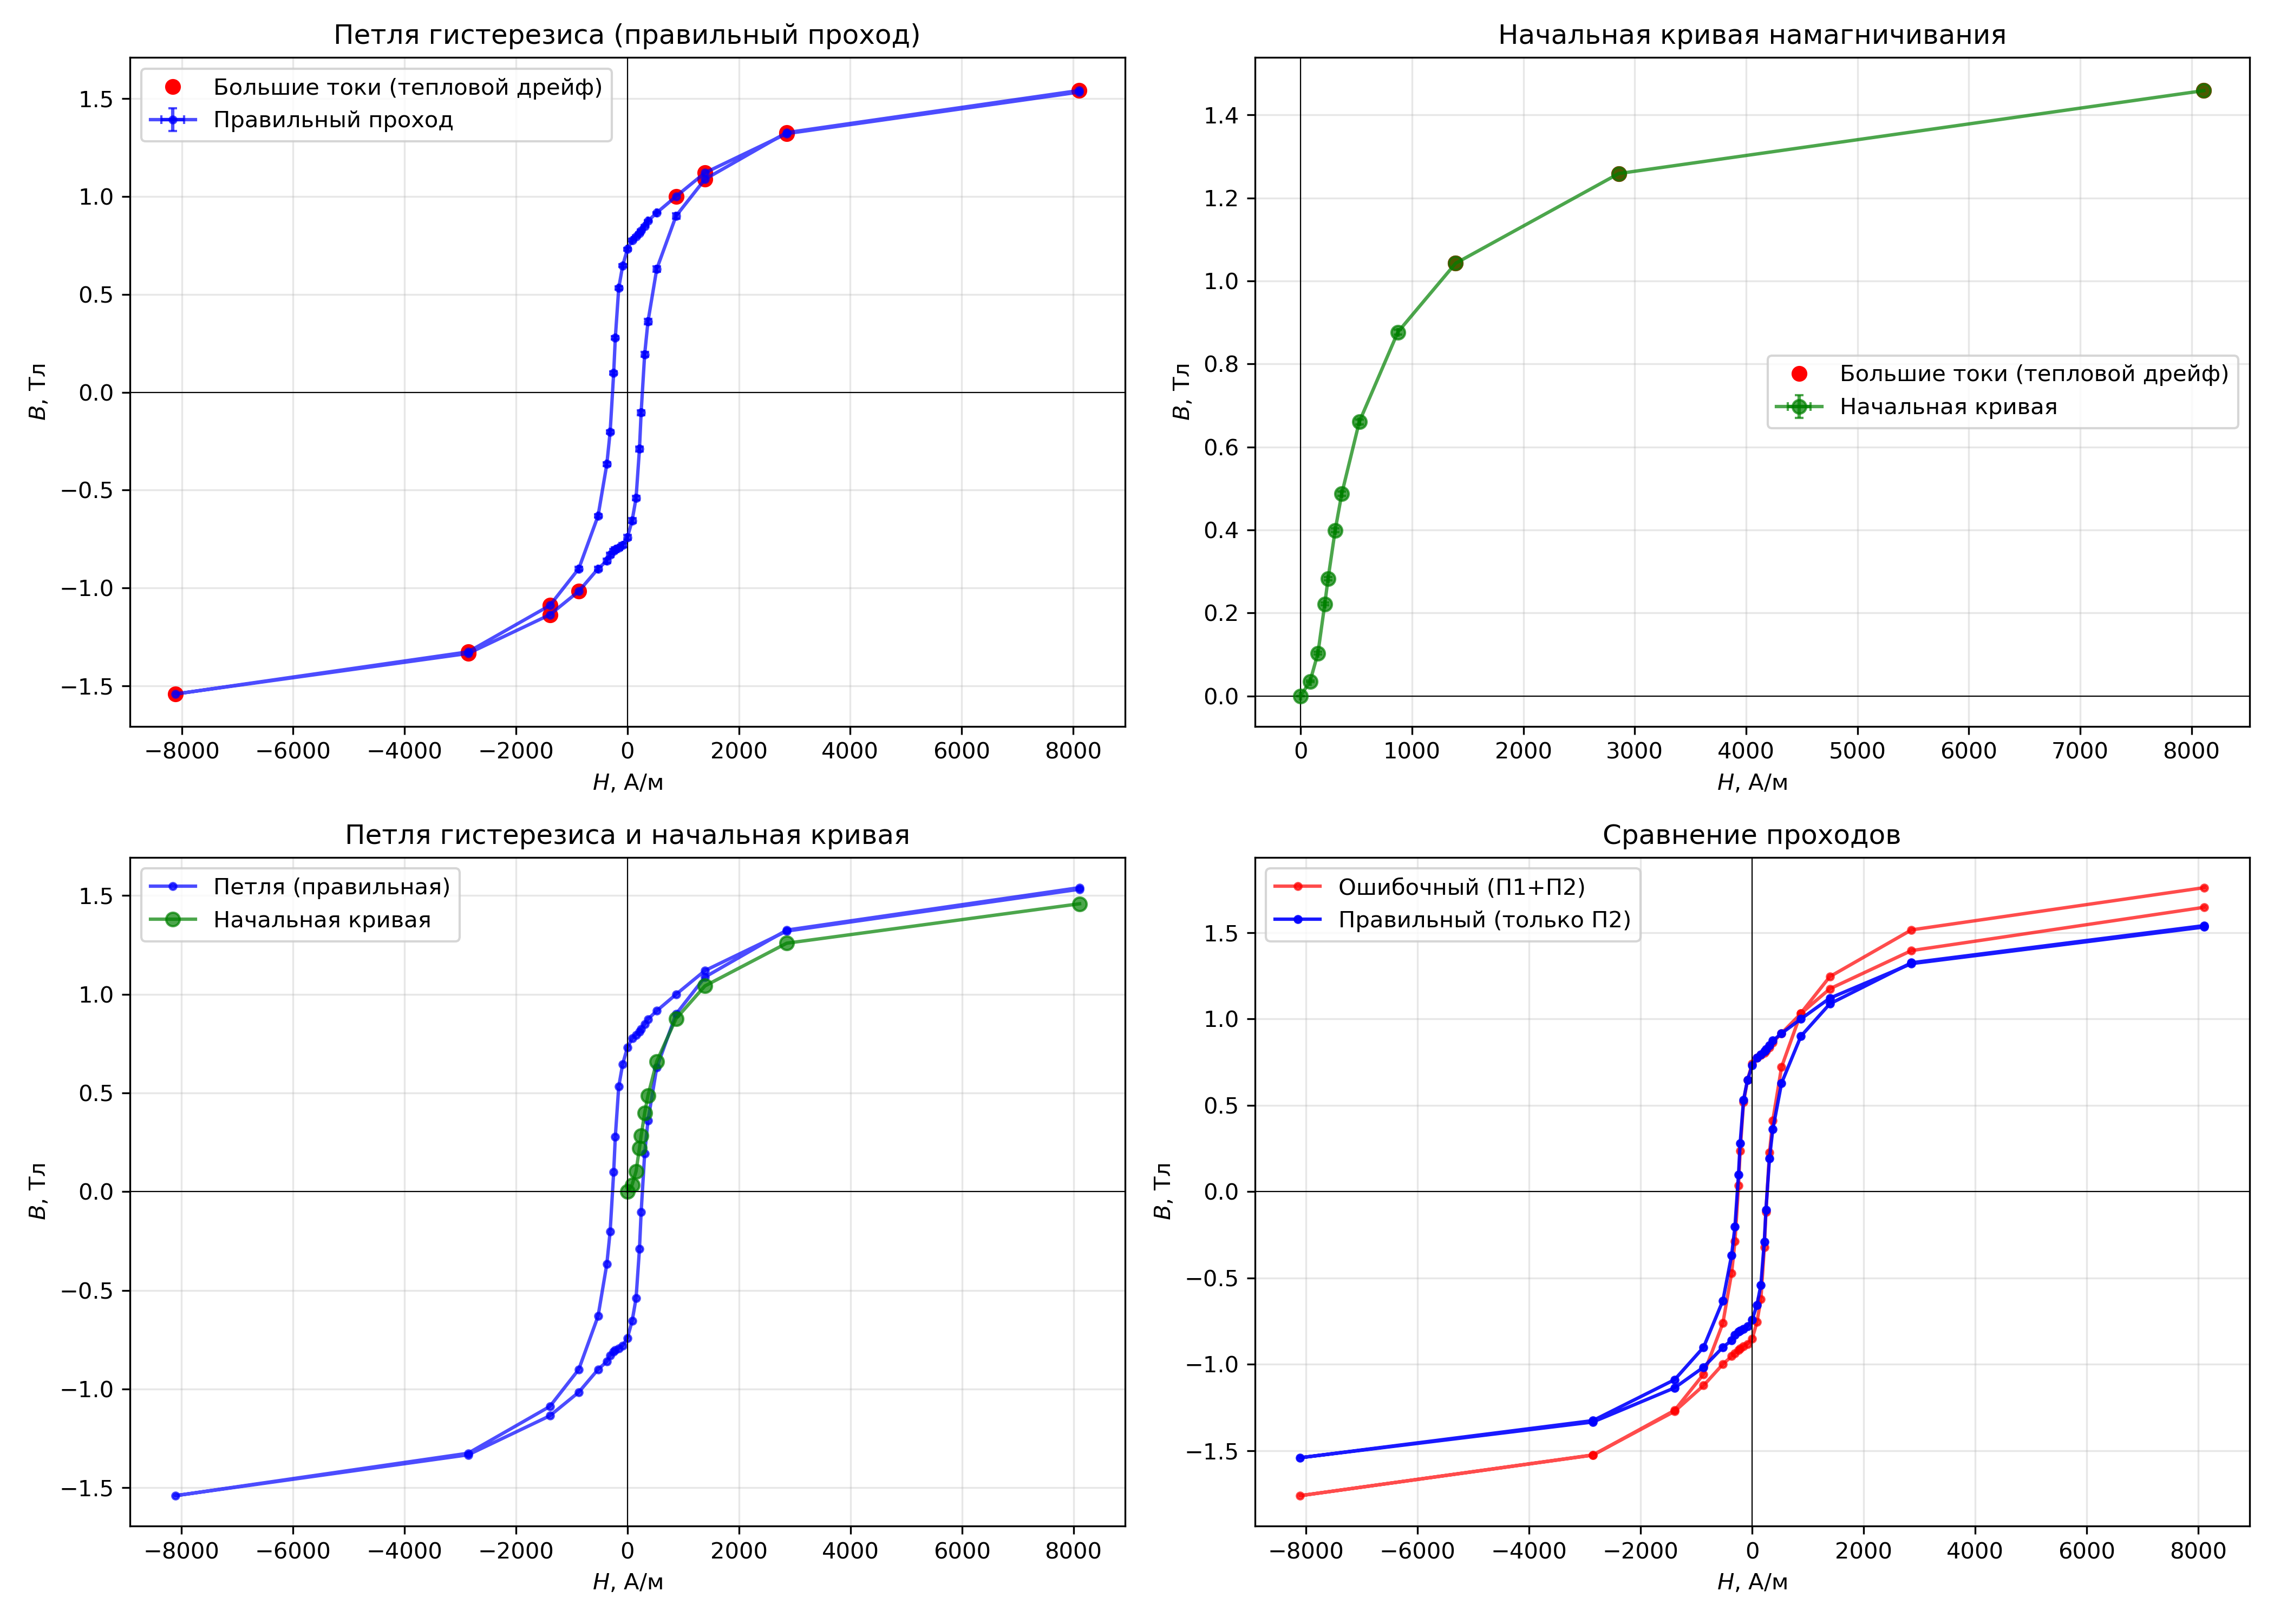
\includegraphics[width=0.9\textwidth]{hysteresis_plots.png}
		\caption{Петля гистерезиса (правильный проход), начальная кривая намагничивания и сравнение проходов. Красным выделены точки, полученные при больших токах (тепловой дрейф)}
		\label{fig:comparison}
	\end{figure}
	
\end{document}